This chapter shows some of the basec algorithms and implementations required to solve problems that include graphs.

\section{Depth First Search (DFS)}

The DFS algorithm is a recursive algorithm that visits all the nodes of a graph. It is used to find connected components, topological sorting, and to find bridges and articulation points. The algorithm is as follows:

\begin{algorithm}
\caption{Depth First Search (DFS)}
\label{alg:dfs}
\begin{algorithmic}[1]
\Procedure{DFS}{$G$}
\State $visited \gets \emptyset$
\State $time \gets 0$
\State $parent \gets \emptyset$
\State $low \gets \emptyset$
\State $disc \gets \emptyset$
\State $AP \gets \emptyset$
\State $bridge \gets \emptyset$
\ForAll{$v \in V$}
\State $visited[v] \gets false$
\State $parent[v] \gets -1$
\State $low[v] \gets \infty$
\State $disc[v] \gets \infty$
\EndFor
\ForAll{$v \in V$}
\If{$visited[v] = false$}
\State DFSUtil($G$, $v$, $visited$, $time$, $parent$, $low$, $disc$, $AP$, $bridge$)
\EndIf
\EndFor
\EndProcedure
\Procedure{DFSUtil}{$G$, $v$, $visited$, $time$, $parent$, $low$, $disc$, $AP$, $bridge$}
\State $visited[v] \gets true$
\State $disc[v] \gets time$
\State $low[v] \gets time$
\State $time \gets time + 1$
\State $children \gets 0$
\ForAll{$u \in Adj(v)$}
\If{$visited[u] = false$}
\State $parent[u] \gets v$
\State $children \gets children + 1$
\State DFSUtil($G$, $u$, $visited$, $time$, $parent$, $low$, $disc$, $AP$, $bridge$)
\State $low[v] \gets min(low[v], low[u])$
\If{$parent[v] = -1$ and $children > 1$}
\State $AP[v] \gets true$
\EndIf
\If{$parent[v] != -1$ and $low[u] \geq disc[v]$}
\State $AP[v] \gets true$
\EndIf
\If{$low[u] > disc[v]$}
\State $bridge[v][u] \gets true$
\EndIf
\Else
\State $low[v] \gets min(low[v], disc[u])$
\EndIf
\EndFor
\EndProcedure
\end{algorithmic}
\end{algorithm}

The implementation can be done as follows:

\lstinputlisting{../Graphs/DFS.cpp}

An application of this algorithm in order to find the shorteast path between two nodes can be done as follows:


\lstinputlisting{../Graphs/DFS-application.cpp}

\section{Breadth First Search (BFS)}

The BFS algorithm is a non-recursive algorithm that visits all the nodes of a graph. It is used to find connected components, topological sorting, and to find bridges and articulation points, to better understand it, a propagating fire can be imagined. The algorithm is as follows:

\begin{algorithm}
\caption{Breadth First Search (BFS)}
\label{alg:bfs}
\begin{algorithmic}[1]
\Procedure{BFS}{$G$}
\State $visited \gets \emptyset$
\State $time \gets 0$
\State $parent \gets \emptyset$
\State $low \gets \emptyset$
\State $disc \gets \emptyset$
\State $AP \gets \emptyset$
\State $bridge \gets \emptyset$
\ForAll{$v \in V$}
\State $visited[v] \gets false$
\State $parent[v] \gets -1$
\State $low[v] \gets \infty$
\State $disc[v] \gets \infty$
\EndFor
\ForAll{$v \in V$}
\If{$visited[v] = false$}
\State BFSUtil($G$, $v$, $visited$, $time$, $parent$, $low$, $disc$, $AP$, $bridge$)
\EndIf
\EndFor
\EndProcedure
\Procedure{BFSUtil}{$G$, $v$, $visited$, $time$, $parent$, $low$, $disc$, $AP$, $bridge$}
\State $visited[v] \gets true$
\State $disc[v] \gets time$
\State $low[v] \gets time$
\State $time \gets time + 1$
\State $children \gets 0$
\ForAll{$u \in Adj(v)$}
\If{$visited[u] = false$}
\State $parent[u] \gets v$
\State $children \gets children + 1$
\State BFSUtil($G$, $u$, $visited$, $time$, $parent$, $low$, $disc$, $AP$, $bridge$)
\State $low[v] \gets min(low[v], low[u])$
\If{$parent[v] = -1$ and $children > 1$}
\State $AP[v] \gets true$
\EndIf
\If{$parent[v] != -1$ and $low[u] \geq disc[v]$}
\State $AP[v] \gets true$
\EndIf
\If{$low[u] > disc[v]$}
\State $bridge[v][u] \gets true$
\EndIf
\Else
\State $low[v] \gets min(low[v], disc[u])$
\EndIf
\EndFor
\EndProcedure
\end{algorithmic}
\end{algorithm}

The implementation can be done as follows:

%\inputminted{c++}{Graphs/BFS.cpp}
\lstinputlisting{../Graphs/BFS.cpp}

%\VerbatimInput{Graphs/BFS.cpp}

\section{Finding Bridges and Articulation Points}

The following algorithms are used to find bridges and articulation points in a graph. The implementation of these algorithms is done using DFS and BFS. This algoithms are based on Tarjan's algorithm.

Tarjan's algorithm is an algorithm that is used to find bridges and articulation points in a graph. The algorithm is as follows:

\begin{algorithm}
\caption{Tarjan's Algorithm}
\label{alg:tarjan}
\begin{algorithmic}[1]
\Procedure{Tarjan}{$G$}
\State $visited \gets \emptyset$
\State $time \gets 0$
\State $parent \gets \emptyset$
\State $low \gets \emptyset$
\State $disc \gets \emptyset$
\State $AP \gets \emptyset$
\State $bridge \gets \emptyset$
\ForAll{$v \in V$}
\State $visited[v] \gets false$
\State $parent[v] \gets -1$
\State $low[v] \gets \infty$
\State $disc[v] \gets \infty$
\EndFor
\ForAll{$v \in V$}
\If{$visited[v] = false$}
\State TarjanUtil($G$, $v$, $visited$, $time$, $parent$, $low$, $disc$, $AP$, $bridge$)
\EndIf
\EndFor
\EndProcedure
\Procedure{TarjanUtil}{$G$, $v$, $visited$, $time$, $parent$, $low$, $disc$, $AP$, $bridge$}
\State $visited[v] \gets true$
\State $disc[v] \gets time$
\State $low[v] \gets time$
\State $time \gets time + 1$
\State $children \gets 0$
\ForAll{$u \in Adj(v)$}
\If{$visited[u] = false$}
\State $parent[u] \gets v$
\State $children \gets children + 1$
\State TarjanUtil($G$, $u$, $visited$, $time$, $parent$, $low$, $disc$, $AP$, $bridge$)
\State $low[v] \gets min(low[v], low[u])$
\If{$parent[v] = -1$ and $children > 1$}
\State $AP[v] \gets true$
\EndIf
\If{$parent[v] != -1$ and $low[u] \geq disc[v]$}
\State $AP[v] \gets true$
\EndIf
\If{$low[u] > disc[v]$}
\State $bridge[v][u] \gets true$
\EndIf
\Else
\State $low[v] \gets min(low[v], disc[u])$
\EndIf
\EndFor
\EndProcedure
\end{algorithmic}
\end{algorithm}

\lstinputlisting{../Graphs/Tarjan_y_BlockCutTree.cpp}

\subsection{Bridges}

A bridge is an edge that if it is removed, the graph will be divided into two or more components. The implementation is:

\lstinputlisting{../Graphs/FindBridges.cpp}


\subsection{Articulation Points}

An articulation point is a node that if it is removed, the graph will be divided into two or more components. The implementation is:

\lstinputlisting{../Graphs/FindArticulationPoints.cpp}

\section{Flows}

The flow is a concept that is used in many algorithms, it is used to find the maximum flow that could go through a system of nodes.

\subsection{Dinic}

The Dinic algorithm is a useful algorithm to find the maximum flow that could go through a system of nodes. The implementation of this algorithm is:

\lstinputlisting{../Graphs/Dinic.cpp}

This implementation is done in order to do the Dinic algorithm for a graph with a large number of nodes.

This algorithm is based on the idea of the BFS algorithm, it is used to find the shortest path between two nodes, in this case, the shortest path between the source and the sink. The algorithm is as follows:

\begin{algorithm}
\caption{Dinic}
\label{alg:dinic}
\begin{algorithmic}[1]
\Procedure{Dinic}{$G$}
\State $visited \gets \emptyset$
\State $time \gets 0$
\State $parent \gets \emptyset$
\State $low \gets \emptyset$
\State $disc \gets \emptyset$
\State $AP \gets \emptyset$
\State $bridge \gets \emptyset$
\ForAll{$v \in V$}
\State $visited[v] \gets false$
\State $parent[v] \gets -1$
\State $low[v] \gets \infty$
\State $disc[v] \gets \infty$
\EndFor
\ForAll{$v \in V$}
\If{$visited[v] = false$}
\State DinicUtil($G$, $v$, $visited$, $time$, $parent$, $low$, $disc$, $AP$, $bridge$)
\EndIf
\EndFor
\EndProcedure
\Procedure{DinicUtil}{$G$, $v$, $visited$, $time$, $parent$, $low$, $disc$, $AP$, $bridge$}
\State $visited[v] \gets true$
\State $disc[v] \gets time$
\State $low[v] \gets time$
\State $time \gets time + 1$
\State $children \gets 0$
\ForAll{$u \in Adj(v)$}
\If{$visited[u] = false$}
\State $parent[u] \gets v$
\State $children \gets children + 1$
\State DinicUtil($G$, $u$, $visited$, $time$, $parent$, $low$, $disc$, $AP$, $bridge$)
\State $low[v] \gets min(low[v], low[u])$
\If{$parent[v] = -1$ and $children > 1$}
\State $AP[v] \gets true$
\EndIf
\If{$parent[v] != -1$ and $low[u] \geq disc[v]$}
\State $AP[v] \gets true$
\EndIf
\If{$low[u] > disc[v]$}
\State $bridge[v][u] \gets true$
\EndIf
\Else
\State $low[v] \gets min(low[v], disc[u])$
\EndIf
\EndFor
\EndProcedure
\end{algorithmic}
\end{algorithm}

\subsection{Ford Fulkerson}

The Ford Fulkerson algorithm is a useful algorithm to find the maximum flow that could go through a system of nodes. The implementation of this algorithm is:

\lstinputlisting{../Graphs/FordFulkerson.cpp}

In order to better understand the adjecency matrix in the code Figure \ref{fig:ford_fulkerson} shows the graph that is used in the code.

\begin{figure}[h]
\centering
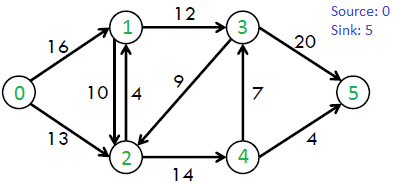
\includegraphics[width=0.35\textwidth]{../Figures/ford_fulkerson11.png}
\caption{Ford Fulkerson}
\label{fig:ford_fulkerson}
\end{figure}

\section{Dijkstra}

The Dijkstra algorithm is a useful algorithm to find the shortest path between two nodes. The implementation of this algorithm is:

\lstinputlisting{../Graphs/Dijkstra.cpp}

Another implementation of this algorithm is the one that is done using a priority queue, the implementation of this algorithm is:

\lstinputlisting{../Graphs/Dijkstra-Mod.cpp}

\section{Bellman Ford}

The Bellman Ford algorithm is a useful algorithm to find the shortest path between two nodes. Bellman Ford diferenctiates from Dijkstra in the fact that it can be used in graphs with negative edges. The algorithm is as follows:

\begin{algorithm}
\caption{Bellman Ford}
\label{alg:bellman_ford}
\begin{algorithmic}[1]
\Procedure{BellmanFord}{$G$}
\State $dist \gets \emptyset$
\State $parent \gets \emptyset$
\ForAll{$v \in V$}
\State $dist[v] \gets \infty$
\State $parent[v] \gets -1$
\EndFor
\State $dist[s] \gets 0$
\For{$i = 0$ to $|V| - 1$}
\ForAll{$v \in V$}
\ForAll{$u \in Adj(v)$}
\If{$dist[u] > dist[v] + w(v, u)$}
\State $dist[u] \gets dist[v] + w(v, u)$
\State $parent[u] \gets v$
\EndIf
\EndFor
\EndFor
\EndFor
\ForAll{$v \in V$}
\ForAll{$u \in Adj(v)$}
\If{$dist[u] > dist[v] + w(v, u)$}
\State $dist[u] \gets -\infty$
\State $parent[u] \gets -1$
\EndIf
\EndFor
\EndFor
\EndProcedure
\end{algorithmic}
\end{algorithm}

The implementation of this algorithm is:

\lstinputlisting{../Graphs/BellmanFord.cpp}

\section{Hamiltonian Cycle}

The Hamiltonian cycle of undirected graph G <= V , E> is the cycle containing each vertex in V. -If graph contains a Hamiltonian cycle, it is called Hamiltonian graph otherwise it is non-Hamiltonian.

Finding a Hamiltonian cycle in a graph is a well-known problem with many real-world applications, such as in network routing and scheduling.

Hamiltonian Path in an undirected graph is a path that visits each vertex exactly once. A Hamiltonian cycle (or Hamiltonian circuit) is a Hamiltonian Path such that there is an edge (in the graph) from the last vertex to the first vertex of the Hamiltonian Path. Determine whether a given graph contains Hamiltonian Cycle or not. If it contains, then prints the path. Following are the input and output of the required function.
Input: 
A 2D array graph[V][V] where V is the number of vertices in graph and graph[V][V] is adjacency matrix representation of the graph. A value graph[i][j] is 1 if there is a direct edge from i to j, otherwise graph[i][j] is 0.
Output: 
An array path[V] that should contain the Hamiltonian Path. path[i] should represent the ith vertex in the Hamiltonian Path. The code should also return false if there is no Hamiltonian Cycle in the graph.

A Hamiltonian cycle is a cycle that visits every node in the graph. The implementation of this algorithm is:

\lstinputlisting{../Graphs/Hamiltonian.cpp}


\section{Eulerian Cycle}

The problem is same as following question. “Is it possible to draw a given graph without lifting pencil from the paper and without tracing any of the edges more than once”.
A graph is called Eulerian if it has an Eulerian Cycle and called Semi-Eulerian if it has an Eulerian Path. The problem seems similar to Hamiltonian Path which is NP complete problem for a general graph. Fortunately, we can find whether a given graph has a Eulerian Path or not in polynomial time. In fact, we can find it in O(V+E) time. 
Following are some interesting properties of undirected graphs with an Eulerian path and cycle. We can use these properties to find whether a graph is Eulerian or not.

Eulerian Cycle: An undirected graph has Eulerian cycle if following two conditions are true. 

All vertices with non-zero degree are connected. We don’t care about vertices with zero degree because they don’t belong to Eulerian Cycle or Path (we only consider all edges). 
All vertices have even degree.
Eulerian Path: An undirected graph has Eulerian Path if following two conditions are true. 

Same as condition (a) for Eulerian Cycle.
If zero or two vertices have odd degree and all other vertices have even degree. Note that only one vertex with odd degree is not possible in an undirected graph (sum of all degrees is always even in an undirected graph)

An Eulerian cycle is a cycle that visits every edge in the graph. The implementation of this algorithm is:

\lstinputlisting{../Graphs/Eulerian.cpp}